% !TEX encoding = UTF-8 Unicode
\documentclass[
10pt,
aspectratio=169,
]{beamer}
\setbeamercovered{transparent=10}
\usetheme[
%  showheader,
%  red,
  purple,
%  gray,
%  graytitle,
  colorblocks,
%  noframetitlerule,
]{Verona}

\usepackage[T1]{fontenc}
\usepackage[utf8]{inputenc}
\usepackage{lipsum}
%%%%%%%%%%%%%%%%%%%%%%%%%%%%%%%
% Mac上使用如下命令声明隶书字体,windows也有相关方式,大家可自行修改
\providecommand{\lishu}{\CJKfamily{zhli}}
%%%%%%%%%%%%%%%%%%%%%%%%%%%%%%%
\usepackage{tikz}
\usetikzlibrary{fadings}
%
%\setbeamertemplate{sections/subsections in toc}[ball]
\usepackage{xeCJK}
\usepackage{listings}
\usepackage{caption}
\usepackage{subfigure}
\usefonttheme{professionalfonts}
\def\mathfamilydefault{\rmdefault}
\usepackage{amsmath}
\usepackage{multirow}
\usepackage{booktabs}
\usepackage{bm}
\setbeamertemplate{section in toc}{\hspace*{1em}\inserttocsectionnumber.~\inserttocsection\par}
\setbeamertemplate{subsection in toc}{\hspace*{2em}\inserttocsectionnumber.\inserttocsubsectionnumber.~\inserttocsubsection\par}
\setbeamerfont{subsection in toc}{size=\small}
\AtBeginSection[]{%
	\begin{frame}%
		\frametitle{Outline}%
		\textbf{\tableofcontents[currentsection]} %
	\end{frame}%
}

\AtBeginSubsection[]{%
	\begin{frame}%
		\frametitle{Outline}%
		\textbf{\tableofcontents[currentsection, currentsubsection]} %
	\end{frame}%
}

\title{Beamer for BUCT}
\subtitle{A Simple while elegant template}
\author[HS.Peng]{Peng Haosong}
\mail{livion\_i@icloud.com}
\institute[Beijing University of Chemical Technology]{College of Information and Science Technology \\
Beijing University of Chemical Technology}
\date{\today}
\titlegraphic[width=4cm]{logo.png}{}




%%%%%%%%%%%%%%%%%%%%%%%%%%%%%%%%
% ----------- 标题页 ------------
%%%%%%%%%%%%%%%%%%%%%%%%%%%%%%%%



\begin{document}

\maketitle

%%% define code
\defverbatim[colored]\lstI{
	\begin{lstlisting}[language=C++,basicstyle=\ttfamily,keywordstyle=\color{red}]
	int main() {
	// Define variables at the beginning
	// of the block, as in C:
	CStash intStash, stringStash;
	int i;
	char* cp;
	ifstream in;
	string line;
	[...]
	\end{lstlisting}
}
%%%%%%%%%%%%%%%%%%%%%%%%%%%%%%%%
% ----------- FRAME ------------
%%%%%%%%%%%%%%%%%%%%%%%%%%%%%%%%

\section{Basics}
\subsection{Blocks}
\begin{frame}[c]{Blocks}
	
The blocks are shown below
这是一个block
\begin{block}{Regular Block}
	Content of a regular block
\end{block}

\begin{exampleblock}{Example Block}
	Content of an example block
\end{exampleblock}

\begin{alertblock}{Alert block}
	Content of an alert block
\end{alertblock}

\end{frame}	

\subsection{Enumerate \& Overlays}

\begin{frame}[c]{Enumerate \& Overlays}
	
{\large An Example of \texttt{enumerate}}
	\begin{enumerate}[<+->]
		\item First item
		\item Second item
		\item Third item
	\end{enumerate}
\vfill
{\large An Example of \texttt{itemize}}	
	\begin{itemize}[<+->]
	\item First item
	\item Second item
	\item Third item
	\end{itemize}
\end{frame}	

\subsection{Two columns}
\begin{frame}[c]{Two columns}
	
\begin{columns}[onlytextwidth]
	\column{0.4\textwidth}
	Content for column one
	\begin{equation}
	E = mc^2
	\end{equation}
	\column{0.4\textwidth}	
	Content for column two
	\begin{equation}
	F=ma
	\end{equation}
\end{columns}
\end{frame}	

\begin{frame}{分栏:左图右字或者左字右图}
\begin{columns}
	\column{0.5\textwidth}
		\begin{figure}
		\centering
		% Requires \usepackage{graphicx}
		
\includegraphics[width=5cm]{logo}
		\caption{分栏示意图}
	\end{figure}
	\column{0.55\textwidth}
	\small
	这里输入文字
\end{columns}
\end{frame}


\subsection{Figures}
\begin{frame}[c]{Figures}
	\begin{figure}
		\centering
		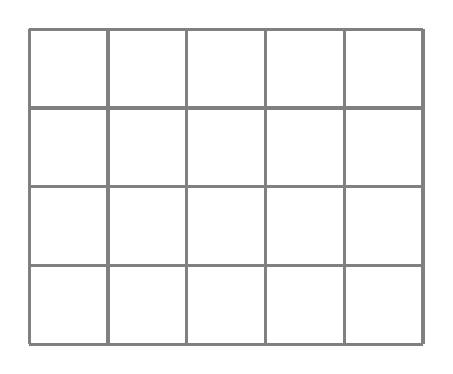
\begin{tikzpicture}
		\draw [help lines,very thick] (0,0) grid (5,4);
		\end{tikzpicture}
		\caption{Credits to Ti\textit{k}Z}
	\end{figure}
\end{frame}	

\begin{frame}{Figures}
怎么插入多张图片:
\begin{figure}[h]
    \centering
    \subfigure[校徽1]{
    
\includegraphics[scale=0.022]{logo.png}
    }
    \subfigure[校徽2]{
    
\includegraphics[scale=0.022]{logo.png}
    }
    \subfigure[校徽3]{
    
\includegraphics[scale=0.022]{logo.png}
    }
    \subfigure[校徽4]{
    
\includegraphics[scale=0.022]{logo.png}
    }
    \caption{demo}
\end{figure}
\end{frame}

\subsection{Code Demo}
\begin{frame}{A Listings Demo}{C++}
	\lstI
\end{frame}

\section{References}

\begin{frame}{BibTex使用}
    这里引用文献\cite{9492070}。
\end{frame}

\begin{frame}{References}
\bibliographystyle{abbrv}     %论文引用格式
\bibliography{References}


\end{frame}
% Thank you page
\beamertemplateshadingbackground{structure.fg!90}{structure.fg}
\begin{frame}[plain]
	\vfill
	\centering
	{
		\centering \Huge \color{white} Thank you for your attention!\\[10pt]Questions?
	}
	\vfill
\end{frame}


\end{document}


